\documentclass[12pt,a4paper]{article}

% ==============================================================================
% CORE PACKAGES & GEOMETRY
% ==============================================================================
\usepackage[margin=0.85in,headheight=15pt]{geometry}
\usepackage[utf8]{inputenc}
\usepackage[T1]{fontenc}
\usepackage{amsmath,amssymb,amsfonts}
\usepackage{booktabs,tabularx,multirow,array}
\usepackage{graphicx}
\usepackage{xcolor}
\usepackage{enumitem}
\usepackage{caption}
\usepackage{subcaption}
\usepackage{fancyhdr}
\usepackage{titlesec}
\usepackage{listings}
\usepackage{url}
\usepackage{float}

% Graphic search paths for project assets and model checkpoint artifacts
\graphicspath{
    {../images/}
    {../models/checkpoints/civicpulse_v2_yolo11m/}
    {images/}
    {models/checkpoints/civicpulse_v2_yolo11m/}
}

% ==============================================================================
% COLOR DEFINITIONS & HYPERLINK SETUP
% ==============================================================================
\definecolor{civicblue}{RGB}{14,75,140}
\definecolor{civicdark}{RGB}{20,30,45}
\definecolor{civicgray}{RGB}{90,100,115}
\definecolor{accentgreen}{RGB}{16,130,70}
\definecolor{codebg}{RGB}{246,248,250}
\definecolor{bordergray}{RGB}{210,215,222}

\usepackage[
    colorlinks=true,
    linkcolor=civicblue,
    citecolor=civicblue,
    urlcolor=civicblue,
    filecolor=civicblue,
    pdfauthor={CivicPulse Engineering Team},
    pdftitle={CivicPulse: AI/ML Technical Documentation},
    pdfsubject={AI-Assisted Monsoon Civic Risk Intelligence & Response System},
    pdfkeywords={YOLO11, ByteTrack, MiDaS, Depth Estimation, PostGIS, Drone Surveillance, Smart Cities}
]{hyperref}

% ==============================================================================
% TYPOGRAPHY & HEADINGS FORMATTING
% ==============================================================================
\titleformat{\section}
  {\normalfont\Large\bfseries\color{civicdark}}{\thesection}{0.8em}{}[\titlerule]
\titleformat{\subsection}
  {\normalfont\large\bfseries\color{civicdark}}{\thesubsection}{0.8em}{}
\titleformat{\subsubsection}
  {\normalfont\normalsize\bfseries\color{civicdark}}{\thesubsubsection}{0.8em}{}

\setlength{\parskip}{0.35em}
\setlength{\parindent}{0pt}

% Header and Footer configuration
\pagestyle{fancy}
\fancyhf{}
\fancyhead[L]{\small\color{civicgray}\textbf{CivicPulse} \textbar\ AI/ML Technical Documentation}
\fancyhead[R]{\small\color{civicgray}ELCIA Smart City Challenge 2026}
\fancyfoot[L]{\small\color{civicgray}Technical Companion Report --- Subsystem Architecture \& Evaluation}
\fancyfoot[R]{\small\color{civicgray}Page \thepage}
\renewcommand{\headrulewidth}{0.4pt}
\renewcommand{\footrulewidth}{0.4pt}

% Code snippet styling
\lstset{
    backgroundcolor=\color{codebg},
    basicstyle=\small\ttfamily,
    breaklines=true,
    frame=single,
    rulecolor=\color{bordergray},
    keywordstyle=\color{civicblue}\bfseries,
    commentstyle=\color{civicgray}\itshape,
    showstringspaces=false,
    tabsize=2
}

% ==============================================================================
% DOCUMENT BEGIN
% ==============================================================================
\begin{document}

% ------------------------------------------------------------------------------
% TITLE BLOCK
% ------------------------------------------------------------------------------
\begin{center}
    {\Huge\bfseries\color{civicdark} CivicPulse}\\[0.2cm]
    {\LARGE\bfseries\color{civicblue} AI/ML Technical Documentation}\\[0.15cm]
    {\large\textit{AI-Assisted Monsoon Civic Risk Intelligence \& Response System}}\\[0.35cm]
    
    \textbf{Challenge Track:} ELCIA Smart City Drone-AI Challenge 2026 \quad\textbullet\quad
    \textbf{Target Zone:} Electronics City (EC-01 to EC-04), Bengaluru\\[0.1cm]
    \textbf{Document Classification:} Technical Companion Report \quad\textbullet\quad
    \textbf{Status:} Implemented \& Experimentally Evaluated
    \vspace{0.3cm}
    \hrule height 1pt
\end{center}

\tableofcontents
\vspace{0.4cm}
\hrule height 0.5pt
\clearpage

% ==============================================================================
% 1. INTRODUCTION
% ==============================================================================
\section{Introduction}

Urban industrial corridors experience rapid, localized infrastructure degradation during monsoon rainfall. Surface water accumulation, asphalt cavities, pavement erosion, stormwater overflow, and displaced utility covers create severe disruption and safety hazards for commuters. Traditional municipal response relies on manual ground surveys and delayed citizen grievance reports, resulting in operational latency and incomplete spatial visibility.

\textbf{CivicPulse} is an automated aerial computer vision and geospatial intelligence platform designed for monsoon civic risk triage. The system ingests raw drone surveillance video accompanied by synchronized SubRip (\texttt{.srt}) flight telemetry, executing a multi-stage machine learning pipeline that converts unstructured aerial footage into geolocated, deduplicated, and severity-scored municipal incident records:
\[
\begin{gathered}
\text{Drone Video + GPS/SRT} \;\longrightarrow\; \text{AI/ML Processing} \;\longrightarrow\; \text{Hazard Detection} \;\longrightarrow\; \text{Tracking / Confirmation} \\
\longrightarrow\; \text{Severity Assessment} \;\longrightarrow\; \text{Geolocation} \;\longrightarrow\; \text{Evidence Generation} \;\longrightarrow\; \text{Civic Incident}
\end{gathered}
\]

By combining pixel-level instance segmentation, multi-frame association tracking, selective relative depth profiling, and spatial database persistence, CivicPulse enforces the foundational operational rule:
\begin{equation}
\boxed{\text{1 Physical Hazard} = \text{1 Incident}}
\end{equation}
This technical companion report documents the models, mathematical formulations, evidence generation mechanisms, empirical evaluation metrics, and current operational boundaries implemented in the repository.

% ==============================================================================
% 2. AI/ML ARCHITECTURE & PROCESSING PIPELINE
% ==============================================================================
\section{AI/ML Architecture \& Processing Pipeline}

The CivicPulse machine learning pipeline is orchestrated by the \texttt{HazardVideoPipeline} class (\path{src/detection/video_tracker.py}). Figure~\ref{fig:architecture} illustrates the system architecture, and Figure~\ref{fig:pipeline} details the core video processing stages.

The pipeline executes eight sequential processing steps:
\begin{enumerate}[leftmargin=1.8em, itemsep=0.15em]
    \item \textbf{Input Ingestion \& Telemetry Extraction}: Reads input drone video (\texttt{.mp4}) and parses the synchronized DJI SRT sidecar. Per-frame timestamps are computed as $t = \text{frame\_idx} / \text{FPS}$ and matched to flight coordinates.
    \item \textbf{Instance Segmentation (YOLO11m-seg)}: Each frame is evaluated by fine-tuned YOLO11m-seg weights, extracting bounding boxes, pixel-level polygon masks, class labels, and confidence scores.
    \item \textbf{Multi-Object Tracking (ByteTrack)}: Associates detections across consecutive frames via two-stage IoU matching, assigning persistent \texttt{track\_id} integers to physical hazards.
    \item \textbf{Temporal Persistence \& Surface Gating}: Requires tracklets to meet per-class hit thresholds ($\text{hits} \ge \text{min\_hits}$) and evaluates optical Laplacian texture variance to reject dry asphalt falsely detected as water.
    \item \textbf{Selective Depth Profiling (MiDaS / DPT-Large)}: Computes relative monocular depth maps selectively on frames where depth-dependent hazards (\texttt{pothole}) are confirmed.
    \item \textbf{Severity Scoring \& Priority Mapping}: Calculates a multi-factor severity score ($0$--$100$) based on surface area coverage percentage and mean relative depth drop, mapping to priority levels ($\text{P1}$, $\text{P2}$, $\text{P3}$).
    \item \textbf{Evidence Generation \& Video Transcoding}: Writes annotated full-resolution snapshot JPEGs (with segmentation masks, bounding boxes, track IDs, and risk tags) and transcodes the complete video stream via FFmpeg (H.264 / \texttt{yuv420p} / \texttt{+faststart}).
    \item \textbf{PostGIS Ingestion \& Dashboard Dispatch}: Ingests detections, evidence file paths, and incident entities into PostgreSQL/PostGIS with spatial geometry points for live operations triage.
\end{enumerate}

\begin{figure}[H]
    \centering
    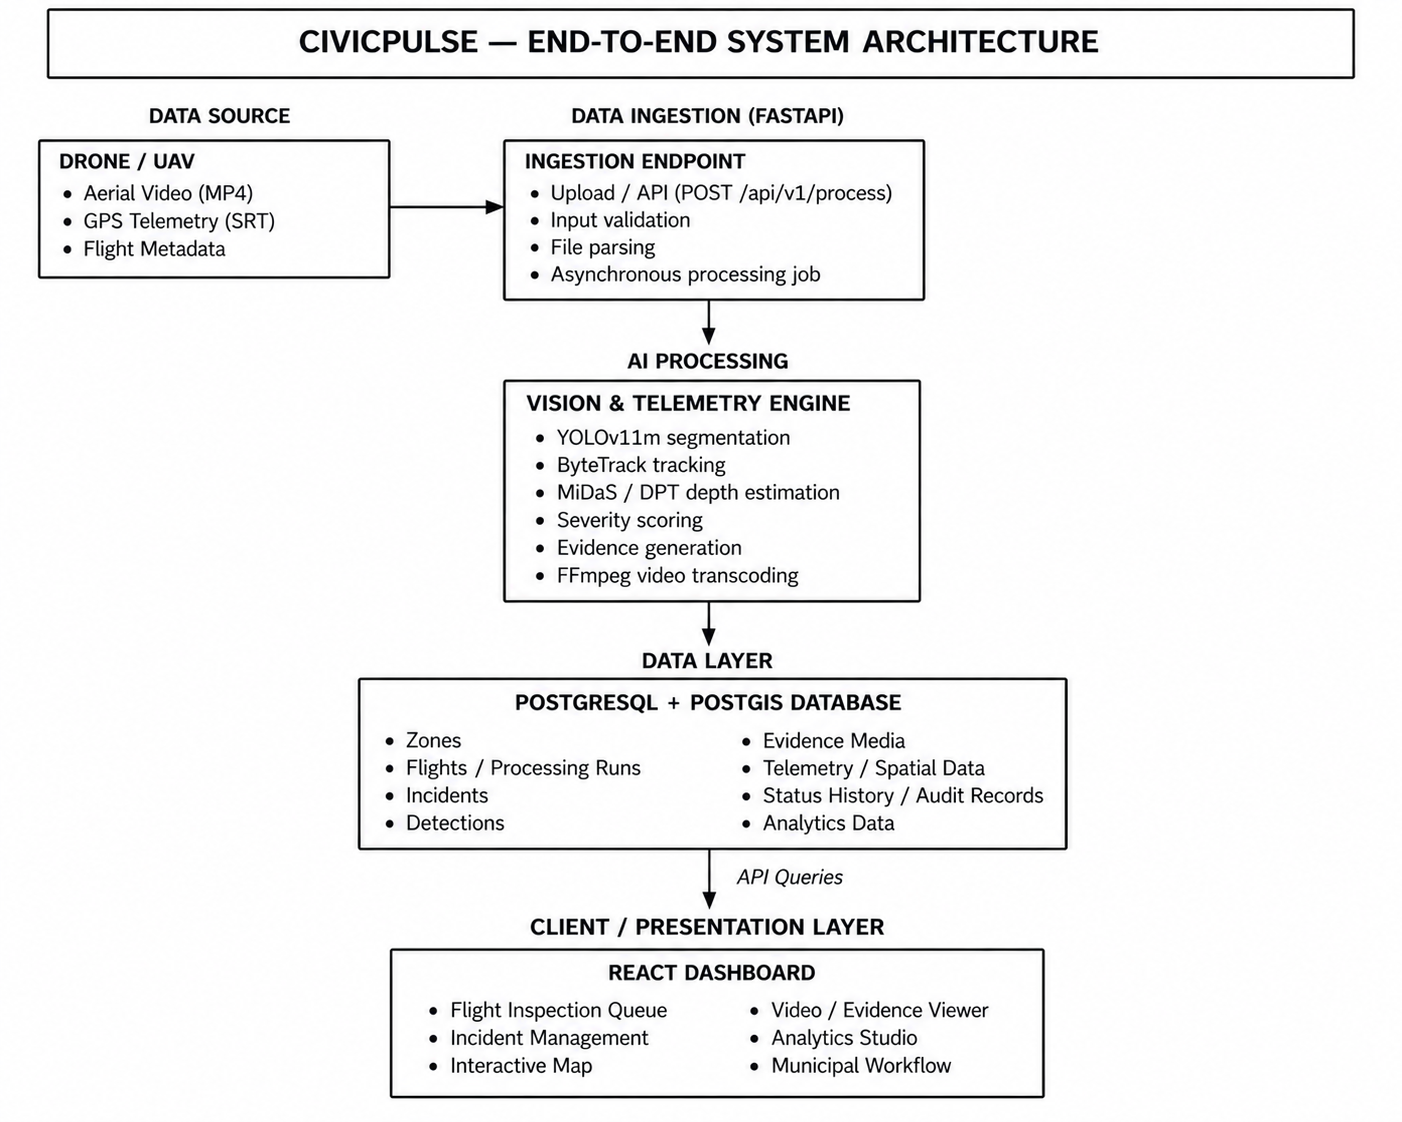
\includegraphics[width=0.88\textwidth]{Architecture.png}
    \caption{CivicPulse System Architecture: Drone Ingestion, AI Vision Engine, PostgreSQL/PostGIS Storage, and React Operations Dashboard.}
    \label{fig:architecture}
\end{figure}

\begin{figure}[H]
    \centering
    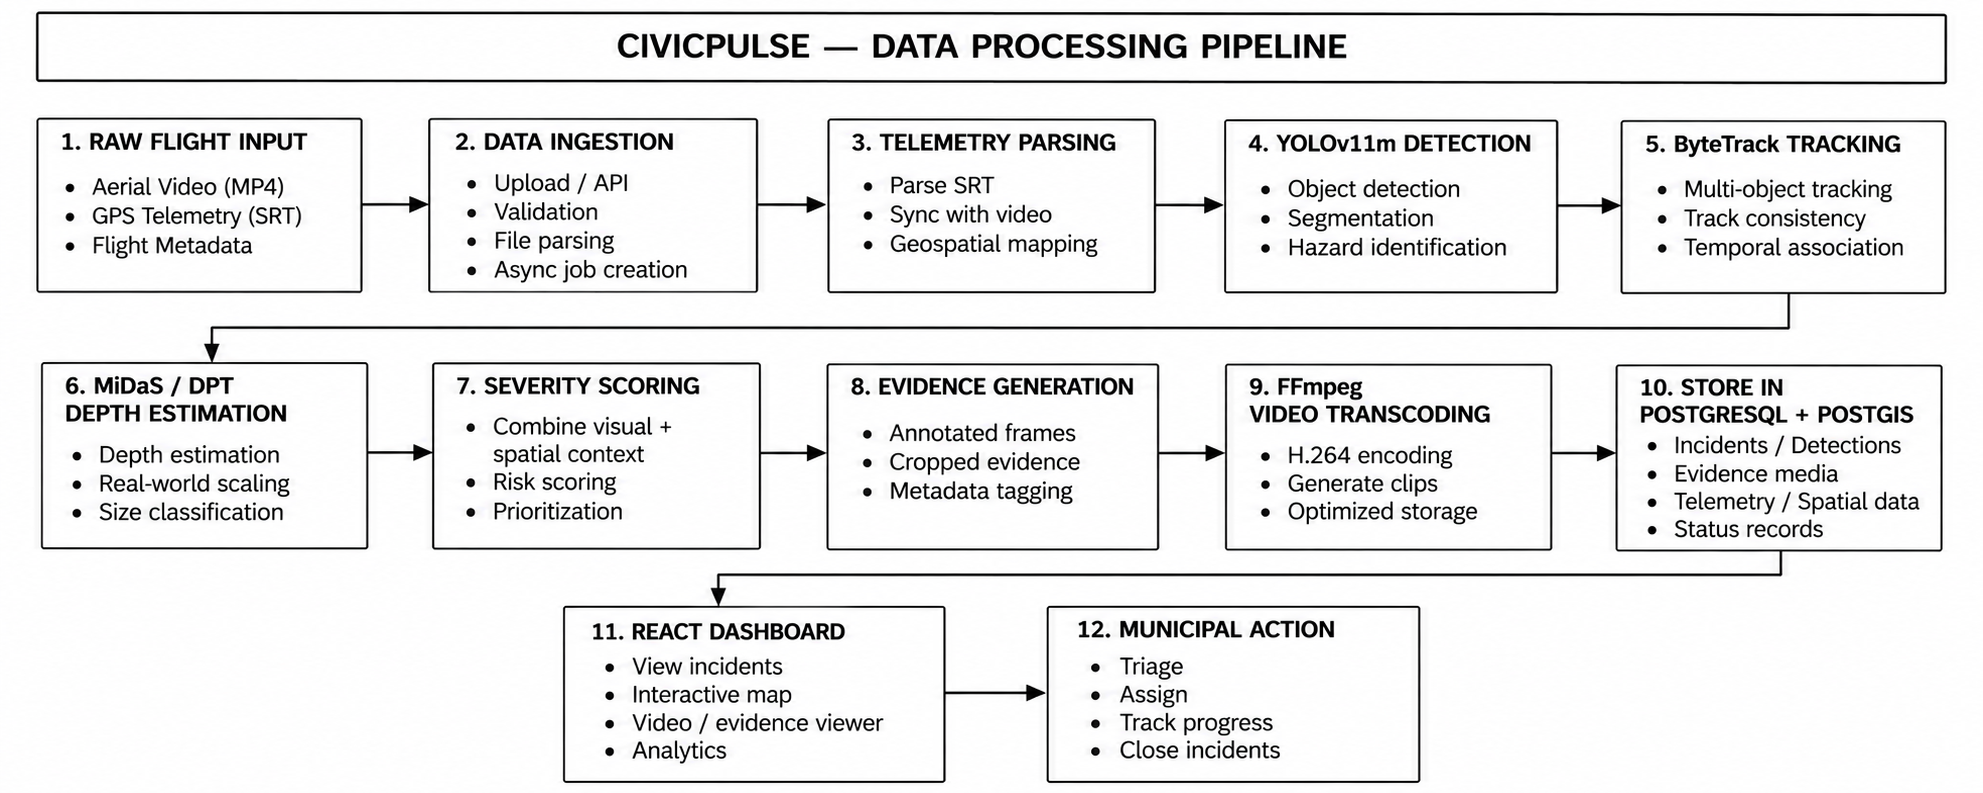
\includegraphics[width=0.88\textwidth]{Pipeline.png}
    \caption{CivicPulse Core Video Processing Pipeline: Sequential frame evaluation, tracking, validation gates, depth profiling, and evidence export.}
    \label{fig:pipeline}
\end{figure}

% ==============================================================================
% 3. INPUT DATA & TELEMETRY
% ==============================================================================
\section{Input Data \& Telemetry}

CivicPulse consumes standard aerial drone surveillance streams. The video stream provides high-resolution spatial frames, while the synchronized SRT sidecar provides per-frame flight telemetry.

\subsection{DJI SRT Telemetry Parsing}
DJI drones record flight telemetry in SubRip subtitle sidecar files (\texttt{.srt}), encoding sequence index, time intervals, and bracketed or legacy coordinate tags:
\begin{lstlisting}[language=text]
1
00:00:00,000 --> 00:00:00,033
[latitude: 12.845214] [longitude: 77.663188] [altitude: 42.5]
\end{lstlisting}

The telemetry parser (\path{scripts/gps_parser.py}) extracts time-indexed GPS points using structured regular expressions supporting both modern bracketed and legacy formats:
\begin{equation}
\text{Pattern}_{\text{new}} = \texttt{\textbackslash[latitude:\textbackslash s*([\textbackslash-\textbackslash d\textbackslash.]+)\textbackslash].*?\textbackslash[longitude:\textbackslash s*([\textbackslash-\textbackslash d\textbackslash.]+)\textbackslash]}
\end{equation}
\begin{equation}
\text{Pattern}_{\text{old}} = \texttt{GPS\textbackslash s*\textbackslash(([\textbackslash-\textbackslash d\textbackslash.]+),\textbackslash s*([\textbackslash-\textbackslash d\textbackslash.]+)\textbackslash)}
\end{equation}

\subsection{Timestamp Association \& Fallback Mechanism}
For each video frame at index $i$ and frame rate $\text{FPS}$, the elapsed flight time in seconds is calculated as:
\begin{equation}
t_i = \frac{i}{\text{FPS}}
\end{equation}

The parser formats $t_i$ into standard \texttt{HH:MM:SS} representation ($\Delta t = \text{str}(\text{timedelta}(\lfloor t_i \rfloor))$) and matches it to the start timestamp of parsed SRT entries. The coordinate matching function operates as follows:
\begin{equation}
\text{GPS}(t_i) = 
\begin{cases}
(\text{lat}_k, \, \text{lon}_k), & \text{if } \text{SRT entry } k \text{ start-time matches } \Delta t \\
(\text{lat}_{\text{last}}, \, \text{lon}_{\text{last}}), & \text{if } t_i > \max(\text{SRT time}) \text{ (tail hold)} \\
(\text{null}, \, \text{null}), & \text{if no SRT file is provided}
\end{cases}
\end{equation}

\textbf{Implementation Note:} Coordinate matching operates via nearest-second prefix matching of subtitle timestamps. The codebase does not perform sub-frame linear geometric spline interpolation. If no SRT telemetry is available, the ingestion service assigns the default centroid of the selected surveillance zone (e.g., \texttt{EC-01}). Table~\ref{tab:data_spec} outlines the supported input/output data schema.

\begin{table}[htbp]
\centering
\small
\caption{CivicPulse Input and Output Data Specifications}
\label{tab:data_spec}
\begin{tabularx}{\textwidth}{l l X}
\toprule
\textbf{Field / Entity} & \textbf{Data Type} & \textbf{Operational Description} \\
\midrule
\texttt{video\_input} & MP4 / MOV & Aerial RGB surveillance video (typically 1080p @ 30 FPS) \\
\texttt{srt\_input} & Text (.srt) & Synchronized DJI telemetry sidecar with GPS coordinates \\
\texttt{frame\_idx} & Integer $\ge 1$ & Monotonically increasing sequential frame index \\
\texttt{timestamp\_sec} & Float (seconds) & Elapsed video timestamp: $t_i = \text{frame\_idx} / \text{FPS}$ \\
\texttt{latitude, longitude} & Float (WGS84) & GPS coordinates mapped to \texttt{PostGIS Point (SRID 4326)} \\
\texttt{track\_id} & Integer $\ge 1$ & ByteTrack multi-frame object association identifier \\
\texttt{class\_name} & Enum (5 classes) & Canonical hazard classification name \\
\texttt{mask\_polygon} & Array of $[x, y]$ & Instance segmentation contour boundary coordinates \\
\texttt{severity\_score} & Integer $[0, 100]$ & Computed multi-factor civic risk score \\
\texttt{evidence\_file} & JPEG Image & Full annotated frame snapshot saved on hazard confirmation \\
\bottomrule
\end{tabularx}
\end{table}

% ==============================================================================
% 4. OBJECT DETECTION --- YOLOV11M
% ==============================================================================
\section{Object Detection --- YOLOv11m}

CivicPulse utilizes a fine-tuned \textbf{YOLO11m-seg} instance segmentation model (\path{models/production/best.pt}) to detect and segment road infrastructure defects. Instance segmentation was chosen over standard bounding-box object detection because municipal road defects (such as sprawling waterlogging patches, irregular asphalt cavities, and meandering drainage overflow streams) have irregular geometric boundaries. Bounding boxes encompass substantial healthy asphalt, distorting surface area calculations, whereas segmentation polygon masks isolate the exact defective footprint.

\subsection{Hazard Classes and Configured Thresholds}
The model is configured for five standardized civic hazard classes defined in \path{configs/config.yaml}:
\begin{enumerate}[leftmargin=1.8em, itemsep=0.1em]
    \item \textbf{\texttt{damaged\_footpath}} (Class 0): Broken walkway pavers, eroded sidewalks ($\tau_{\text{conf}} = 0.15$).
    \item \textbf{\texttt{drainage\_overflow}} (Class 1): Silted stormwater drains, roadside overflow ($\tau_{\text{conf}} = 0.30$).
    \item \textbf{\texttt{open\_manhole}} (Class 2): Missing or displaced utility/sewer access covers ($\tau_{\text{conf}} = 0.60$).
    \item \textbf{\texttt{pothole}} (Class 3): Asphalt cavities and road surface craters ($\tau_{\text{conf}} = 0.30$).
    \item \textbf{\texttt{waterlogging}} (Class 4): Standing rainwater inundation across road corridors ($\tau_{\text{conf}} = 0.30$).
\end{enumerate}

\subsection{Detection Parsing \& Spatial Moments}
For each predicted instance contour $C = \{(x_k, y_k)\}_{k=1}^K$, the polygon surface area in pixels is computed via Green's theorem (implemented in \texttt{cv2.contourArea}):
\begin{equation}
A_{\text{mask}} = \frac{1}{2} \left| \sum_{k=1}^K (x_k y_{k+1} - x_{k+1} y_k) \right|
\end{equation}

Microscopic visual artifacts are rejected by enforcing a minimum area threshold $A_{\text{mask}} \ge 50.0\text{ pixels}$. The spatial centroid $(\bar{x}, \bar{y})$ of the polygon is calculated using spatial image moments $M_{ij} = \sum_{x, y} x^i y^j I(x, y)$:
\begin{equation}
\bar{x} = \frac{M_{10}}{M_{00}}, \qquad \bar{y} = \frac{M_{01}}{M_{00}}
\end{equation}

The detection output tuple passed downstream contains:
\begin{equation}
\mathcal{D} = \left\{ \text{track\_id}, \, \text{class\_id}, \, \text{class\_name}, \, \text{confidence}, \, \text{bbox}, \, (\bar{x}, \bar{y}), \, C, \, A_{\text{mask}}, \, \frac{A_{\text{mask}}}{H \cdot W} \right\}
\end{equation}

% ==============================================================================
% 5. OBJECT TRACKING --- BYTETRACK
% ==============================================================================
\section{Object Tracking --- ByteTrack}

In continuous aerial video, running frame-by-frame object detection without tracking produces repetitive observations of the same physical road defect. A drone hovering over a single pothole for 5 seconds at 30 FPS would generate 150 separate detection instances.

\subsection{Two-Stage Association Formulation}
CivicPulse integrates ByteTrack configured in \path{configs/custom_bytetrack.yaml}. ByteTrack associates detections across consecutive frames by matching both high- and low-confidence boxes:
\begin{itemize}[leftmargin=1.5em, itemsep=0.1em]
    \item \textbf{Stage 1 (High-Confidence Association)}: Detections with confidence score $s \ge \tau_{\text{high}} = 0.20$ are matched to existing active tracks using spatial Intersection over Union (IoU) with threshold $\tau_{\text{match}} = 0.70$:
    \begin{equation}
    \text{IoU}(B_{\text{det}}, B_{\text{track}}) = \frac{\text{Area}(B_{\text{det}} \cap B_{\text{track}})}{\text{Area}(B_{\text{det}} \cup B_{\text{track}})} \ge 0.70
    \end{equation}
    \item \textbf{Stage 2 (Low-Confidence Recovery)}: Unmatched tracks are matched against remaining low-confidence detections ($0.08 \le s < 0.20$) to maintain track identity through camera motion blur or partial occlusion.
    \item \textbf{Track Lifecycle}: Unmatched high-confidence detections ($s \ge \tau_{\text{new}} = 0.22$) initialize new tracklets. Lost tracklets are buffered for $\text{track\_buffer} = 60\text{ frames}$ ($\sim 2.0\text{ seconds}$ at 30 FPS) before deletion.
\end{itemize}

\subsection{Validation Gating \& Persistence Verification}
Before a tracklet is confirmed as an official incident, it must satisfy two validation gates:
\begin{enumerate}[leftmargin=1.8em, itemsep=0.1em]
    \item \textbf{Temporal Persistence Gate}: The track hit counter must satisfy $\text{hits} \ge \text{min\_hits}$. Standard defects require $\text{min\_hits} = 2$; high-priority hazards like \texttt{open\_manhole} require $\text{min\_hits} = 3$; \texttt{waterlogging} requires $\text{min\_hits} = 5$ to reject transient puddles.
    \item \textbf{Optical Laplacian Texture Variance Gate}: Fresh, dark asphalt can visually mimic standing water. For hazards with \texttt{requires\_smooth\_surface: true} (\texttt{waterlogging}), the region of interest (ROI) is evaluated via the variance of the Laplacian operator:
    \begin{equation}
    \sigma^2_{\text{Laplacian}} = \text{Var}\left(\nabla^2 I_{\text{gray}}(\text{ROI})\right) = \text{Var}\left(\frac{\partial^2 I}{\partial x^2} + \frac{\partial^2 I}{\partial y^2}\right)
    \end{equation}
    True standing water exhibits specular, optically smooth surfaces ($\sigma^2 < 550.0$), whereas dry textured asphalt exhibits high structural grain variance ($\sigma^2 > 600.0$). Detections failing this gate are discarded.
\end{enumerate}

% ==============================================================================
% 6. DEPTH ESTIMATION --- MIDAS / DPT
% ==============================================================================
\section{Depth Estimation --- MiDaS / DPT}

To evaluate the vertical depression of road cavities, CivicPulse integrates zero-shot monocular depth estimation using the \textbf{DPT-Large} (Dense Prediction Transformer) architecture (\path{src/detection/depth_estimator.py}).

\subsection{Selective Execution}
Running continuous transformer depth inference on every 1080p frame would severely reduce video processing throughput. Therefore, depth estimation is executed \textbf{selectively}: it triggers exclusively on the confirmation frame of depth-dependent classes (\texttt{pothole}, configured with \texttt{needs\_depth: true} in \path{configs/config.yaml}).

\subsection{Mathematical Representation}
The DPT model processes the frame image and outputs an inverse relative disparity map $d(x, y)$. This map is interpolated to native frame dimensions $(H, W)$ via bicubic interpolation and min-max normalized to uint8 $[0, 255]$:
\begin{equation}
d_{\text{norm}}(x, y) = 255 \times \frac{d(x, y) - \min(d)}{\max(d) - \min(d)}
\end{equation}

The mean relative depth score $\bar{d}_{\text{rel}} \in [0.0, 1.0]$ over the hazard's binary polygon mask $M_{\text{poly}}$ is computed as:
\begin{equation}
\bar{d}_{\text{rel}} = \frac{1}{|M_{\text{poly}}|} \sum_{(x, y) \in M_{\text{poly}}} \frac{d_{\text{norm}}(x, y)}{255.0}
\end{equation}

\textbf{Operational Note:} Monocular depth estimation provides \textbf{relative optical disparity} within the visual frame context. It indicates relative indentation intensity compared to surrounding road pixels and is not a metric depth measurement calibrated in physical centimeters.

% ==============================================================================
% 7. SEVERITY & RISK ASSESSMENT
% ==============================================================================
\section{Severity \& Risk Assessment}

CivicPulse calculates an automated multi-factor severity score for every confirmed hazard (\path{src/detection/severity_analyzer.py}).

\subsection{Actual Severity Formulations}
The severity score incorporates surface area coverage percentage $A_{\%}$ and mean relative depth drop $\bar{d}_{\text{rel}}$:
\begin{equation}
A_{\%} = \left(\frac{A_{\text{pixels}}}{H \times W}\right) \times 100
\end{equation}
\begin{equation}
S_{\text{ML}} = \min\left(100, \, \left\lfloor 2 \cdot A_{\%} + 50 \cdot \bar{d}_{\text{rel}} \right\rfloor \right)
\end{equation}

For hazards where depth estimation is not required (e.g., \texttt{damaged\_footpath}, \texttt{waterlogging}), $\bar{d}_{\text{rel}} = 0.0$.

For database persistence and REST API delivery (\path{src/services/ml_ingestion_service.py}), the integer score $S_{\text{ML}} \in [0, 100]$ is normalized to a backend scale of $0.0$--$10.0$:
\begin{equation}
S_{\text{backend}} = \text{round}\left(\frac{S_{\text{ML}}}{10.0}, \, 2\right)
\end{equation}

Table~\ref{tab:severity_rules} details the severity score thresholds, corresponding municipal priority levels, and operational triage workflows.

\begin{table}[htbp]
\centering
\small
\caption{CivicPulse Severity Scores, Risk Levels, and Priority Mapping}
\label{tab:severity_rules}
\begin{tabularx}{\textwidth}{l l l X}
\toprule
\textbf{Risk Level} & \textbf{Condition ($S_{\text{ML}}$)} & \textbf{Priority} & \textbf{Operational Action} \\
\midrule
\textbf{CRITICAL} & $S_{\text{ML}} > 70$ & \textbf{P1} & Immediate emergency barricading; urgent pump/repair dispatch \\
\textbf{MODERATE / HIGH} & $40 < S_{\text{ML}} \le 70$ & \textbf{P2} & Scheduled civil maintenance within 24-hour window \\
\textbf{LOW} & $S_{\text{ML}} \le 40$ & \textbf{P3} & Routine monitoring; added to regular road maintenance queue \\
\bottomrule
\end{tabularx}
\end{table}

% ==============================================================================
% 8. GEOLOCATION & EVIDENCE GENERATION
% ==============================================================================
\section{Geolocation \& Evidence Generation}

\subsection{Spatial Transformation}
When a hazard is confirmed at frame $i$ (elapsed time $t_i$), the GPS parser matches the nearest latitude and longitude $(\text{lat}_i, \text{lon}_i)$. During database ingestion, these coordinates are stored as a spatial geometry point:
\begin{equation}
\text{Geom} = \texttt{ST\_SetSRID(ST\_MakePoint(lon, lat), 4326)}
\end{equation}

\subsection{Evidence Artifact Pipeline}
To support human verification and municipal auditing, CivicPulse generates two evidence artifacts:
\begin{enumerate}[leftmargin=1.8em, itemsep=0.1em]
    \item \textbf{Annotated Evidence Snapshot}: At the confirmation frame, \texttt{draw\_detections()} overlays the semi-transparent segmentation polygon ($\alpha = 0.4$), bounding box, centroid marker, ByteTrack ID, and class confidence tag. The annotated frame is written to disk at:
    \begin{equation}
    \path{outputs/jobs/{job_id}/evidence/hazard_{track_id}_{risk_level}.jpg}
    \end{equation}
    \item \textbf{Progressive H.264 Video Transcoding}: The complete annotated video stream is transcoded via FFmpeg using the H.264 codec, \texttt{yuv420p} pixel format, and \texttt{+faststart} flag:
    \begin{lstlisting}[language=bash]
ffmpeg -y -i raw_stream.mp4 -c:v libx264 -preset fast -crf 22 -pix_fmt yuv420p -movflags +faststart annotated_output.mp4
    \end{lstlisting}
    This enables progressive streaming in the frontend operations dashboard without requiring full-file pre-buffering.
\end{enumerate}

% ==============================================================================
% 9. MODEL EVOLUTION --- YOLOV8S TO YOLO11M
% ==============================================================================
\section{Model Evolution --- YOLOv8s $\rightarrow$ YOLO11m}

CivicPulse evaluated two model checkpoints trained on custom 5-class civic hazard datasets:
\begin{itemize}[leftmargin=1.5em, itemsep=0.1em]
    \item \textbf{v1 Baseline}: \texttt{yolov8s-seg.pt} trained at $1024 \times 1024$ resolution for 143 epochs (early-stopped with patience 30).
    \item \textbf{v2 Current}: \texttt{yolo11m-seg.pt} trained at $640 \times 640$ resolution for 105 epochs (early-stopped with patience 30).
\end{itemize}

\subsection{Experimental Comparison}
Table~\ref{tab:model_comparison} reports the actual validation metrics recorded in the training logs (\path{results.csv}) of both checkpoints. The training convergence curves and normalized confusion matrix are illustrated in Figure~\ref{fig:model_curves}, and the class-specific mask precision-recall curves are shown in Figure~\ref{fig:mask_pr}.

\begin{table}[htbp]
\centering
\small
\caption{Empirical Metric Comparison: YOLOv8s-seg vs. YOLO11m-seg Checkpoint Artifacts}
\label{tab:model_comparison}
\begin{tabularx}{\textwidth}{l c c r}
\toprule
\textbf{Metric} & \textbf{YOLOv8s-seg (v1)} & \textbf{YOLO11m-seg (v2)} & \textbf{Observed Delta} \\
\midrule
\textbf{Base Model Architecture} & \texttt{yolov8s-seg.pt} & \texttt{yolo11m-seg.pt} & Upgraded C3k2/C2PSA blocks \\
\textbf{Training Input Size} & $1024 \times 1024$ & $640 \times 640$ & Standardized batching \\
\textbf{Batch Size / Epochs} & Batch 4 / 143 Epochs & Batch 16 / 105 Epochs & Faster training convergence \\
\midrule
\textbf{Box Precision ($P_B$)} & 0.710 & 0.674 & Adjusted for recall gain \\
\textbf{Box Recall ($R_B$)} & 0.560 & \textbf{0.651} & \textbf{+9.1\%} ($\Delta = +0.091$) \\
\textbf{Box mAP@50} & 0.581 & \textbf{0.649} & \textbf{+6.8\%} ($\Delta = +0.068$) \\
\textbf{Box mAP@50-95} & 0.331 & \textbf{0.361} & \textbf{+3.0\%} ($\Delta = +0.030$) \\
\midrule
\textbf{Mask Precision ($P_M$)} & 0.718 & 0.672 & Adjusted for recall gain \\
\textbf{Mask Recall ($R_M$)} & 0.560 & \textbf{0.670} & \textbf{+11.0\%} ($\Delta = +0.110$) \\
\textbf{Mask mAP@50} & 0.578 & \textbf{0.646} & \textbf{+6.8\%} ($\Delta = +0.068$) \\
\textbf{Mask mAP@50-95} & 0.333 & \textbf{0.345} & \textbf{+1.2\%} ($\Delta = +0.012$) \\
\midrule
\textbf{Validation Box Loss} & 1.752 & \textbf{1.523} & \textbf{--13.1\%} \\
\textbf{Validation Seg Loss} & 2.803 & \textbf{1.644} & \textbf{--41.4\%} \\
\textbf{Validation Cls Loss} & 2.354 & \textbf{1.280} & \textbf{--45.6\%} \\
\bottomrule
\end{tabularx}
\end{table}

\begin{figure}[htbp]
    \centering
    \begin{subfigure}[b]{0.48\textwidth}
        \centering
        \includegraphics[width=\textwidth]{results.png}
        \caption{Training and Validation Metrics vs. Epochs}
        \label{fig:results_curve}
    \end{subfigure}
    \hfill
    \begin{subfigure}[b]{0.48\textwidth}
        \centering
        \includegraphics[width=\textwidth]{confusion_matrix_normalized.png}
        \caption{Normalized Validation Confusion Matrix}
        \label{fig:confusion_matrix}
    \end{subfigure}
    \caption{Experimental Training Artifacts from YOLO11m-seg Checkpoint (\path{civicpulse_v2_yolo11m}): (a) Loss and mAP metric progressions across 105 epochs, and (b) Normalized class confusion matrix showing diagonal true-positive dominance.}
    \label{fig:model_curves}
\end{figure}

\begin{figure}[htbp]
    \centering
    \includegraphics[width=0.55\textwidth]{MaskPR_curve.png}
    \caption{YOLO11m-seg Precision-Recall Curve for Mask Segmentation across 5 Hazard Classes ($\text{mAP@50} = 0.646$).}
    \label{fig:mask_pr}
\end{figure}

\subsection{Evaluation Analysis \& Trade-Offs}
Under the evaluated CivicPulse training configurations, YOLO11m-seg demonstrated significant performance gains over the YOLOv8s-seg baseline:
\begin{enumerate}[leftmargin=1.8em, itemsep=0.1em]
    \item \textbf{Significant Recall Improvement}: As shown in Table~\ref{tab:model_comparison}, mask recall increased from $56.0\%$ to $67.0\%$ ($+11.0\%$), and box recall from $56.0\%$ to $65.1\%$ ($+9.1\%$). In municipal hazard monitoring, higher recall reduces missed road hazards.
    \item \textbf{Precision vs. Recall Trade-Off}: Precision slightly decreased (Box Precision: $0.710 \rightarrow 0.674$, Mask Precision: $0.718 \rightarrow 0.672$) as the model captured more edge cases. As seen in Figure~\ref{fig:mask_pr}, this trade-off favors overall detection coverage across diverse municipal conditions.
    \item \textbf{Reduced Validation Losses}: As tracked in Figure~\ref{fig:results_curve}, validation classification loss dropped by $45.6\%$ ($2.354 \rightarrow 1.280$) and segmentation loss by $41.4\%$ ($2.803 \rightarrow 1.644$), demonstrating improved class discrimination and mask localization. The confusion matrix in Figure~\ref{fig:confusion_matrix} confirms high separation among the five civic hazard categories.
\end{enumerate}

\textbf{Experimental Context:} The YOLOv8s and YOLO11m runs differed in training image size ($1024$ vs $640$), batch size ($4$ vs $16$), and data augmentation configurations. Therefore, observed improvements reflect the combined benefits of the model upgrade, hyperparameter tuning, and dataset refinements rather than an isolated architecture change. Inference latency on uniform edge hardware was not benchmarked in these runs.

% ==============================================================================
% 10. CURRENT RESULTS & LIMITATIONS
% ==============================================================================
\section{Current Results \& Limitations}

\subsection{Implementation Status}
\begin{itemize}[leftmargin=1.5em, itemsep=0.1em]
    \item \textbf{IMPLEMENTED}: End-to-end video processing pipeline, DJI SRT telemetry parser, YOLO11m instance segmentation, ByteTrack multi-object association, selective DPT-Large depth profiling, automated multi-factor severity analyzer, annotated evidence JPEG export, H.264 video transcode, and PostgreSQL/PostGIS spatial persistence.
    \item \textbf{EXPERIMENTALLY EVALUATED}: YOLOv8s-seg vs. YOLO11m-seg performance across 5 hazard classes on training/validation splits with exact CSV metrics and confusion matrix artifacts.
    \item \textbf{PLANNED}: TensorRT INT8 model export, calibrated metric depth estimation using stereo/LiDAR hardware, and multi-spectral thermal/NIR sensor fusion.
\end{itemize}

\subsection{Software Validation}
Separate from machine learning metrics, the software codebase maintains rigorous automated test coverage:
\begin{itemize}[leftmargin=1.5em, itemsep=0.1em]
    \item \textbf{Backend Test Suite (Pytest)}: \textbf{147 passing tests} covering database migrations, API routes, repository queries, spatial conversions, and evidence snapshot generation.
    \item \textbf{Frontend Test Suite (Vitest)}: \textbf{123 passing tests (13 test suites)} verifying incident queues, state machine transitions, video playback seeking, and analytics calculations.
\end{itemize}

\subsection{Current Limitations}
\begin{enumerate}[leftmargin=1.8em, itemsep=0.1em]
    \item \textbf{Relative vs. Metric Depth}: Monocular depth estimation outputs relative inverse disparity rather than calibrated metric millimeters. It provides qualitative cavity rankings within a single frame context.
    \item \textbf{Telemetry Dependency}: Spatial accuracy relies on the presence and precision of DJI SRT flight subtitles. Videos without SRT telemetry fall back to operational zone defaults.
    \item \textbf{Environmental Domain Variations}: Severe downpours, low-light dusk flights, and direct sun specular glint on wet surfaces introduce visual domain shifts that can affect detection confidence.
    \item \textbf{Compute Requirements}: Selective DPT-Large depth estimation and 1080p video tracking require GPU acceleration (NVIDIA CUDA or Apple Silicon MPS) for near-real-time throughput.
\end{enumerate}

\subsection{Next Steps}
\begin{itemize}[leftmargin=1.5em, itemsep=0.1em]
    \item \textbf{Edge Quantization}: Export YOLO11m-seg to TensorRT and ONNX INT8 formats for onboard drone companion computer execution.
    \item \textbf{Metric Depth Calibration}: Integrate stereoscopic cameras or LiDAR sensors to produce physical cavity depth measurements in metric units.
    \item \textbf{Multi-Spectral Fusion}: Evaluate thermal infrared and near-infrared (NIR) imaging to detect subsurface waterlogging before surface inundation occurs.
\end{itemize}

\end{document}
